\documentclass[a4paper, 10pt]{article}
\usepackage{fullpage} % changes the margin
\usepackage[english]{babel}
\usepackage[utf8]{inputenc}
\usepackage{hyperref}
\usepackage{xcolor}
\usepackage{graphicx}
\usepackage{array}
\usepackage{float}
\usepackage{longtable}
\usepackage[bottom]{footmisc}
\usepackage{cite}
\usepackage{parskip}
\usepackage{subcaption}
\usepackage{amssymb}
\usepackage{amsmath}
\usepackage{listings}
\usepackage{titlesec}

\hypersetup{
	colorlinks=true,       % false: boxed links; true: colored links
	linkcolor=blue,        % color of internal links
	citecolor=blue,        % color of links to bibliography
	filecolor=magenta,     % color of file links
	urlcolor=blue
}

% TEMPLATE SETTINGS
\setlength{\parindent}{0cm}
\setlength{\parskip}{2mm}
\renewcommand{\baselinestretch}{1.2}
\titlespacing*{\section}
{0pt}{2mm}{2mm}
\titlespacing*{\subsection}
{0pt}{1.2mm}{1.2mm}

%\setlength{\parindent}{0cm}
\newcommand{\code}[1]{\texttt{#1}}
\renewcommand{\arraystretch}{1.2}

\graphicspath{{../plots/}}

\begin{document}

\noindent
\begin{flushright}
	\large\textbf{Miguel Alcón Doganoc} \\
	Multiprocessors Architecture \\
	%\today
	June 29, 2020
\end{flushright}
\vspace{2mm}
\noindent
{\huge{\textbf{State-of-the-art in the design and certification process of Autonomous Driving systems}}}
\vspace{-3mm}

In the past few years, there have been lots of research and development in both industry and academia about the design and certification of Autonomous Driving (AD) systems. Safety-critical systems are typically control systems whose design and verification is data-independent, and data is mostly used for validation in the form of tests. However, AD systems, which are safety-critical real-time systems, increasingly build on deep learning, whose implementation relies on systems designed together with training data sets, thus making data (including training dataset for deep learning models) part of the design and verification phase, which is against the design and verification principles in safety standards. Recently, there has been some research activity in this direction, trying to fill the gap between the emerging challenges that the complexity of AD systems impose on their design and certification process. In this work, I give some insights on the latest research about this topic.

%Our objective in this project is to study the latest research and provide a survey of the most promising works that have been done.

\section{Challenges in Autonomous Vehicle Testing and Validation~\cite{challenges}}
The development process of safety-related automotive systems is well-defined in the ISO 26262, the main functional safety standard for road vehicles. The ISO 26262 development V process (see Figure~\ref{fig:v}) sets up a framework that ties each type of testing to a corresponding design or requirement document. It represents a methodical process of creation followed by verification and validation. The left side of the V works its way from requirements through design to implementation. Instead, its right side iteratively verifies and validates larger and larger chunks of the system as it climbs back up from small components to a system-level assessment. 
\begin{figure}[htbp]
	\centering
	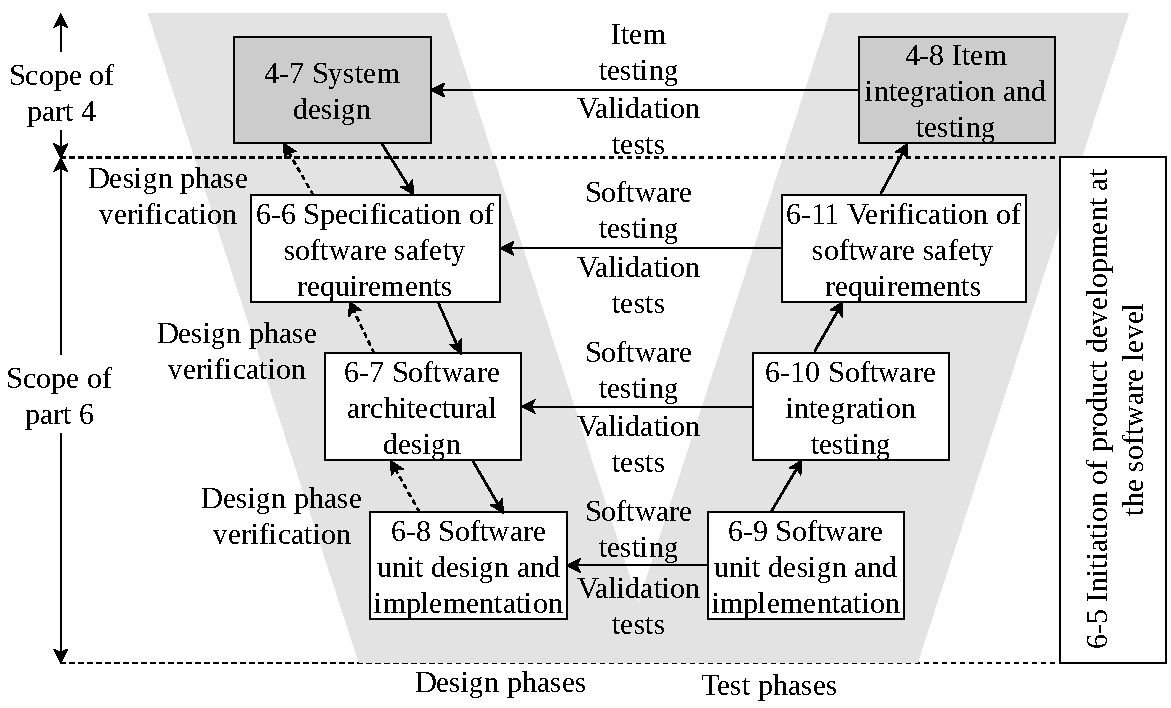
\includegraphics[width=0.7\linewidth]{figures/Part6development.pdf}
	\caption{The ISO 26262 development V process (picture taken from \cite{En-Route:SAC2020}).}
	\label{fig:v}
\end{figure}

The problem here is that ISO 26262 presents challenges when adapted to deal with the sorts of novel testing issues that face autonomous vehicles (AV), and AVs cannot be considered safe unless and until they are shown to conform or map to ISO 26262 or some other suitable, widely accepted software safety standard. For this reason, the paper discussed in this section identifies five major challenge areas in testing according to the V model for AVs: driver out of the loop, complex requirements, non-deterministic algorithms, inductive learning algorithms, and fail-operational systems. %The paper also identifies the general solution approaches that seem promising across these different challenge areas: phased deployment using successively relaxed operational scenarios, use of a monitor/actuator pair architecture to separate the most complex autonomy functions from simpler safety functions, and fault injection as a way to perform more efficient edge case testing.

\subsection{Driver Out of the Loop}
\label{ssec:driver}
The hardest challenge in a fully AV is dealing with the fact that the driver is no longer driving the vehicle, which means that the driver cannot be counted on to provide control inputs to the vehicle during operation. This is a tough challenge since typical automotive safety arguments for low-integrity devices hinge upon the ability of a human driver to exert control. For instance, with an Advanced Driver Assistance System (ADAS), if a software fault causes a potentially dangerous situation, the driver might be expected to over-ride that software function and recover to a safe state. Situations in which the driver does not have an ability to take corrective action are said to lack controllability, and thus must be designed to a higher Automotive Safety Integrity Level (ASIL). Each element of an AV is attached to an ASIL, which specifies the element's necessary safety requirements for achieving an acceptable residual risk. The ASIL ranges from A to D, where D is the most stringent safety level and A the least.

One way to handle a potentially high-ASIL autonomy function is to use ASIL decomposition via a combination of a monitor/actuator architecture and redundancy. In a monitor/actuator architecture, the primary functions are performed by one module (the actuator), and a paired module (the monitor) performs an acceptance test or validation to the results of the first, thus checking the correct behaviour of the actuator. If the actuator misbehaves, the monitor shuts both modules down, resulting in a fail-silent system (i.e., any failure results in a silent component). If the monitor/actuator pair is designed correctly, the actuator can be designed to a low ASIL whether the monitor has a sufficiently high ASIL and detects all possible faults in the monitor. However, this kind of architecture causes loss of the actuator function if something goes wrong, which is a problem for a function that cannot fail operationally, such as steering in a moving vehicle. Hence, once the system detects that some of the autonomy functions are not working properly, it must somehow bring itself to a safe state.

\subsection{Complex Requirements}
\label{ssec:requirements}
As explained before, removing the driver from the control system implies that the system itself has to handle exceptions. These exceptions can be the consequence of different situations, such as bad weather, traffic rule violations, local driving conventions, or animal hazards. Even each of these situations can happen simultaneously. The challenge presented here is that the system's requirements should be clear about what is within the scope of its design, as well as what is not. However, AVs have simply too many requirements to enumerate in a classical written requirements specification. Thus, it seems unlikely that a classical V process that starts with a document that enumerates all system requirements will be scalable to AV exception handling in a rigorous way, at least in the immediate future.

One way to manage the complexity of requirements is to constrain operational concepts and engage in a phased expansion of requirements. For instance, limiting operational concepts to specific road access, visibility, vehicular environment, external environment, or speed. This is already being done by developers who might concentrate on-road testing in particular geographic regions, thus limiting the the weather the AV can be exposed to and the roads or highways it can navigate on, which determines the speed limit too.

Once sufficient confidence is gained regarding the requirements for a particular operational concept, additional similar operational concepts can be added over time to expand the envelope of allowable automation scenarios. This will not entirely eliminate the issue of complex requirements, but it can help mitigate the combinatorial explosion of requirements and exceptions that would otherwise occur.

\subsection{Non-Deterministic and Statistical Algorithms}
Some of the technologies used in AVs are inherently statistical in nature. In general, they tend to be non-deterministic, giving answers that are only correct to some probability. Validating such systems presents challenges not typically found in traditional automotive control systems. One possible problem to face when performing a vehicle-level test is the fact that, in the same scenario, the process under evaluation could potentially lead to a different outcome despite attempts to exercise nominally identical test cases. Moreover, classification algorithms (e.g., selecting the type of obstacle the AV is facing, such as pedestrians, cars or cyclists), which are non-deterministic, exhibit a tradeoff between false negatives and false positives, with fewer of one necessarily incurring more of the other. The testing implications of this are that the results of these algorithms can be incorrect and, depending on construction, they might report a particular situation as being true when there is only a moderately high probability of that situation actually being true.
%, and they can ne very sensitive to small changes in the initial conditions.

Handling non-determinism in testing is difficult for at least two reasons. The first is that it can be challenging to exercise a particular specific edge-case situation. This can occur because the system might behave in a way that activates an edge case only if it receives a very specific sequence of inputs from the world, which could be hard due to factors discussed earlier. The second is that it can be tough to evaluate whether test results are correct or not, because there is no unique correct system behaviour for a given test case. For this reason, testing non-deterministic algorithms is likely to take a a lot of more tests than simple functional validation, especially if the behaviour in question is safety-critical and expected to have an extremely low failure rate.

%Probabilistic system behaviors present a similar challenge to validation, because passing a test once does not mean that the test will be passed every time. Therefore, testing might not be oriented toward determining if behaviors are correct, but rather to validating that the statistical characteristics of the behaviour are accurately specified.

\subsection{Machine Learning Systems}
Machine learning algorithms build a mathematical model based on sample data (known as \textit{training data}), in order to make predictions or decisions without being explicitly programmed to do so. Validating this training data is an open question that might be addressed by some combination of characterizing the data as well as the data generation or data collection processes.

Because of the complexity of requirements for an autonomous system, it seems likely that rare, edge cases will be where learning problems could occur. However, because of their rarity, collecting data depicting such unusual circumstances can be expensive and difficult to scale. So, simulation and synthetic data could be considered for these cases, but they could lead to other problems. To this, we can add another challenge, commonly known as the \textit{black swan} problem, which is, in general, the susceptibility of a person (or system) to believe that common observations are the only true, and draw potentially incorrect conclusions due to an abundance of confirming
data points. Another obstacle developers have to face is the fact that humans cannot intuitively understand the results of the learning process (e.g., the internal structure of a neural network). This makes it hard to predict how techniques, other than expensive brute force testing, can be applied for validation of machine learning systems.

Validating an inductive learning system seems to be an extremely challenging problem. Extensive testing might be used, but would require validating an assumption of random independent arrival rates of \textit{black swan} data (unusual cases) and testing on data sets sized accordingly. This might be feasible given enough resources, but there will always be new \textit{black swans}, so a probabilistic assessment of huge numbers of operational scenarios and input values would have to be made to ensure an acceptably low level of system failures. An alternative to validating inductive learning systems to high ASIL levels would be to pair a low-ASIL inductively-based algorithm that sends commands to an actuator with a high-ASIL deductively-based monitor. This would sidestep the majority of the validation problem for the actuation algorithm, since failures of the inductive algorithm controlling the actuator would be caught by a non-inductive monitor based on a concept such as a deductively-generated safety envelope. Thus, actuator algorithm failures would be an availability problem (the system safety shuts down, assuming an adequate failover capability) rather than a safety problem.

\subsection{Fail-Operational Systems}
Retaking what has been discussed in section~\ref{ssec:driver}, if the computer is ultimately in control of the vehicle rather than a human driver, at least some portion of it has to be fail-operational instead of fail-stop. In other words, the AV cannot stop working until it is in a safe state. Fail-operational systems need redundancy, so when one component fails, another one can take over. Achieving this requires at least two independent, redundant subsystems for fail-stop behaviour. For instance, commercial aircraft are commonly configured with two jet engines, and each jet engine has at least a dual-redundant computer control. If the pair of computers on one engine shuts down due to a fault detected via continual crosschecking, there is a second independent engine to keep the aircraft flying until reaching its destination. The travel between when a fault is detected and the system reaches a safe state is called failover mission. In the case of AVs, they do have an advantage in that failover missions can be short (e.g., pull over to the side of the road), with durations measured in seconds rather than hours. This can simplify requirements complexity, computational redundancy, sensor requirements, and validation requirements. Therefore, designing an AV with a fail-stop primary controller and a simpler fail-operational failover controller might be attractive both in terms of hardware cost and in terms of design/validation cost.

\subsection{Conclusions}
The challenges of developing safe AVs according to the ISO 26262 V process are significant. However, it is required for ensuring that AVs are safe. Assuming that the V process is applied, there are three general approaches that seem promising. The first is a \textbf{phased deployment} approach building on current developer practice, which can be done by identifying well-specified operational concepts to limit the scope of operations and so the necessary scope of requirements. As shown in section~\ref{ssec:requirements}, this includes limitations in the environment, system health, and operational constraints that must be satisfied to enable autonomous operation. The second is the use of a \textbf{monitor/actuator architecture}. As discussed, this architectural style can help with requirements complexity (higher ASIL devoted to the monitor instead of the actuator), and deployment of inductive learning algorithms (by limiting the use of induction to the actuator, and using a deductively-based monitor). The third is \textbf{fault injection}, which can be used to validate functionality and  to probe for weak spots that might be activated via unforeseen circumstances.


\section{Autonomous Vehicles Testing Methods Review~\cite{methods}}
Following the previous chapter, the inherent and growing complexity of AD systems challenges the testing and validation processes of AVs, which are a required task before their deployment. Moreover, checking the safety of AD systems in critical situations can be a cumbersome task. However, we currently have good references for virtual or real approaches used in ADAS and AD domains for testing such methods. One of these approaches is virtual simulation testing, from simulated sensors, vehicle dynamic model and controller, virtual driver, to simulated comprehensive traffic environment. Another approach is real traffic driving tests. The advantage of simulation in front of real traffic testing is that the first is simpler, costs less, and is easier to reproduce. On the other hand, the reliability of simulated testing results is highly depended on the accuracy of simulated sensors, vehicle and environment models. So, although on-road testing is very representative, it has limited ability to test all critical scenarios due to safety and costs involved. For all this reasons, the paper discussed in this section reviews the existing methods of AD functional testing, verification and validation.

\subsection{Autonomous Driving Testing Related Methods}
Software testing on AD systems has to handle a million lines of code, which require functional automation test on source code level and also require enhanced security of permanently online safety-critical systems. At the same time, such testing requires automatically created test cases, hardware-in-the-loop (HIL) testing, change-based testing and the mapping of tests cases to requirements, such as ISO26262.

Another approach to consider is the simulation testing and, when applied on AD systems, it must be high-fidelity. The dedicated software containing a mathematical representation of the subsystems should be used in order to achieve a realistic system dynamic, which can be validated with HIL techniques. Currently, there are several simulators that can be used by these tasks, such as Racer, USARSim, CarMaker, SUMO, PreScan and SiVIC. Each of them has its advantages and inconveniences. For instance, SUMO and USARSim have been actually used to simulate AVs in a traffic environment, but lacks detailed testing methods elements, especially in driving environmental perception.

Last but not least, AV can be tested in real traffic scenarios, on open environments. There are currently AV cars, like the ones developed by Google (Waymo), that are being tested in real traffic. In fact, test drives with prototype vehicles are always the final
link in the validation chain to evaluate the system's performance in the real-world environment where it will finally be used. In addition, a good methodology to test and validate or assess automated or autonomous vehicles is using real pre-crash scenarios based on experimental data. For example, Volvo's pedestrian detection system is evaluated based on real-life accidents.

\subsection{Autonomous Vehicle Functional Testing}
The architecture of an V is based on general driver behaviour. It follows a sensor-based and actuator-based autonomous system architecture, consisting of Perception, Decision, Navigation and Action layers. 

The Perception layer is responsible for processing all the data from sensors, which includes gathering the raw data, transforming it into computer-readable data, and merging the result (from all sensors) into a unique fusion map. By physical tests, software test or HIL simulation test, both the various sensors and environment Perception layer are tested. 

The Decision layer is fed by the Perception layer providing feedback data to optimize the data acquisition further and interprets all incoming data from it to generate a reasonable output to the Action layer. Artificial Intelligence (AI) algorithms are commonly used in the Decision layer because of the highly non-linear behaviour of the real environment. The evaluation of AV decision making modules is done by way of test drive or simulation test. The driving system reaction characteristic are used for indicators, such as reaction time and operating correctness.


The Navigation layer performs higher-level tasks related to driving, such as controlling the global objectives, trajectory planning, efficiency and commodity, taking into account the driving conditions. This layer is also tested by test drive or simulation.

Finally, the Action layer receives commands through the Decision layer into the action's supervisor, which sets up the abstract decision into set points to be fed by the actuators' controllers. The vehicle trajectory deviation, acceleration and jitter are used to evaluate this layer and, again, the evaluation is done by test drive or simulation.	

\subsection{Autonomous Vehicle Evolutionary Testing Method}
\subsubsection{Autonomous Vehicle Evolutionary Design and Testing Flow}
The AV development starts with a definition of the functional requirements in terms of the desired functions, from the basic AD functional requirements to handle short term and long term planning, avoid dangerous collision and driving safety obey the traffic rules, and with further constraints or requirements on safety, mobility, passenger comfort, and intelligent operational. 

AVs are safety-critical systems that require a high level of dependability, a term covering reliability, fail-safety, and fault-tolerance. In addition to the system safety, it requires driving safety, identify the safety requirements, with criteria indicators of driving gaps, velocity and trajectory control. At the same time, AVs should compliant with the operating efficiency, driving comfort requirements, with criteria indicators of lateral and longitudinal velocity, acceleration and jitter. All these functional requirements have to be defined at the start of the AV's development phase, and they form the AV system specification.

The system specification is used as the basis for the top-level design of the system architecture, followed by detailed perception, planning and control modules design with environment sensor, controller, actuator, driver autopilot etc. After implementation of the individual hardware and software modules, system integration takes place by assembling the complete system from its component modules. In every integration phase, verification takes place to determine whether the output of a phase meets its specification.

On the modules level, every function should be tested, to validate the perception systems, planning and control logic of such AVs using simulation and virtual techniques and HIL by different novel test approach. On the sensors and perception level, this means testing the range, accuracy, and tracking capabilities of the environment sensor. On the control level, this means testing the vehicle stability and control accuracy. On the planning level, this means the trajectory evaluation against the obstacles and other vehicles. The hardware controller can be tested in a HIL simulation for its real-time behaviour. This limited HIL setup can gradually be extended to include other modules, as the integration of the vehicle progresses.

\subsubsection{Evolutionary Autonomous Vehicle System Testing Methods}
Testing AV in real traffic has its limitations because test results are hard to reproduce and sometimes are inaccurate. It happens due to the complexity of getting the true state of the obstacles, pedestrians and the other vehicles involved in the test. For this reason, long test mileages are required to perform a full coverage of the scenarios. One possible solution that can be applied is to combine the advantages of simulations with the representativeness of test drives (mixed reality methods), by extending the HIL environment from vehicle level to the traffic level.

Using mixed reality methods, one can accelerate AV testing and validation, thus reducing the costs of these kinds of processes. In such methods, the validation is firstly carried out in simulation environments, which are built from real traffic scenarios. Then, the driving test is performed in the corresponding real environment. After that, the simulation models of various components can be corrected with real feedback, thus overcoming the problem of simulation model inaccuracy. Since the simulation environment can be easily reconstructed and configured with scenario auto-generation tools, it is a good way to solve the problem of the full coverage of traffic scenarios. Furthermore, AV behaviour in traffic accident scenarios can be simulated and evaluated, which is very helpful during the AD system development.

\subsection{Conclusions}
AV testing is a critical step in the deployment of AD systems. It is necessary to integrate the existing methods, bring out a complete set of methods for AD testing for different stages of the development process, and provide reliable, quick, safe, low cost and reproducible testing methods to accelerate the development.

\section{Final conclusion}
\vspace{-1mm}
Both papers tackle the problem of verifying and validating AD systems. The first~\cite{challenges} explain where the complexity of such processes comes from, and gives some possible solutions to those problems. To sum up, the challenges a developer has to face when verifying or validating AVs are: (1) the system can no longer count with the human driver taking the control when some failure occurs; (2) there are an uncountable number of possible exceptions that difficult the specification of the requirements; (3) the inherent nature of non-deterministic algorithms and (4) machine learning systems complicates the verification and validation tasks; and (5) the system must guide the AV to a safe state after a failure occurs. The second~\cite{methods} some insights on what methods can be used to test AVs. They put emphasis on the comparison of the pros and cons of real traffic testing vs simulated testing. In the end, the authors encourage the usage of the fusion of both kind of testing methods, which they called mixed reality methods. It benefices from the best of both worlds, thus dealing with the inaccuracy of the simulated scenarios and the lack of repeatability of real situations.

Before finishing with this document, I would like to mention that some of the explanations I put on it, to clarify some points of the reviewed papers, are taken from the work I did at the Barcelona Supercomputing Center, which can be summarized in \cite{En-Route:SAC2020} and \cite{TimingApollo:RTAS2020}.

\vspace{-1mm}
\bibliographystyle{plain}
\bibliography{cite}


\end{document}